\documentclass[11pt,a4paper]{article}

\usepackage[margin=1in]{geometry}
\usepackage{graphicx}
\usepackage{booktabs}
\usepackage{amsmath}
\usepackage[hidelinks]{hyperref}

\title{\textbf{JetGraph: Graph Neural Networks for Quark/Gluon Jet Tagging}}
\author{Mohamed Yanis IDIR}
\date{\today}

\begin{document}

\maketitle

\begin{abstract}
JetGraph is a compact high-energy physics and machine-learning study of
quark/gluon jet tagging with particle-level jet constituents. Using the
EnergyFlow \texttt{qg\_jets} dataset, the project compares interpretable
physics-inspired observables with graph neural networks based on EdgeConv.
Observable-only baselines already provide strong discrimination, with gradient
boosting reaching ROC AUC 0.8616. A first EdgeConv model trained on
k-nearest-neighbour particle graphs reaches comparable performance, with the
best hybrid node-feature setup reaching ROC AUC 0.8617 on the Pythia test set.
Additional ablations study feature representation, graph connectivity,
particle-identity information, and Pythia-vs-Herwig generator dependence.
\end{abstract}

\section{Introduction}

Quark/gluon tagging is a standard benchmark problem for studying jet
substructure and machine-learning methods in collider physics. The task is
challenging because jets are variable-size sets of particles, and because useful
discrimination can arise from both global radiation patterns and local
particle-level correlations.

JetGraph is designed as a reproducible mini-study of this problem. The analysis
starts with simple physics observables, then moves to particle-level graph
representations and a small graph neural network. This staged structure makes
the comparison scientifically interpretable: the graph model is judged not only
by its raw performance, but also by whether it improves on meaningful physics
baselines and remains stable under controlled ablations.

\section{Physics Motivation}

Jets are collimated sprays of hadrons produced by energetic partons. Gluon jets
typically radiate more than quark jets because gluons carry a larger color
factor. As a result, gluon-initiated jets tend to have higher particle
multiplicity, broader angular radiation, and different energy-sharing patterns.
These properties motivate observables such as multiplicity, jet mass, and
angular widths.

Graph neural networks offer a complementary representation. Instead of reducing
the jet to a few global quantities, they operate on the particle cloud itself.
This is close to the physical picture of a jet as a structured set of
constituents, and is related to successful particle-cloud architectures such as
ParticleNet~\cite{qu2020particlenet}.

\section{Dataset}

The study uses the EnergyFlow \texttt{qg\_jets} dataset~\cite{komiske2019energyflow}.
The primary sample contains 10,000 Pythia jets generated for quark/gluon
classification. Each event is represented as a padded array of particle
constituents with columns
\[
  (p_T, \eta, \phi, \mathrm{pid}) .
\]
Padded particles are removed by requiring $p_T > 0$. Herwig samples are used in
the generator-robustness study.

\section{Physics-Inspired Baseline Observables}

The baseline model uses five global jet observables:
\begin{itemize}
  \item particle multiplicity, excluding padded constituents;
  \item scalar constituent $p_T$ sum;
  \item approximate jet mass from massless constituent four-vectors;
  \item $p_T$-weighted $\eta$ width;
  \item $p_T$-weighted $\phi$ width.
\end{itemize}
These quantities encode the expected differences between quark and gluon
radiation patterns. Logistic regression, random forest, and gradient boosting
are trained on these observables.

\section{Graph Construction}

For the graph-based model, each jet is converted into a PyTorch Geometric
\texttt{Data} object~\cite{fey2019pyg}. Nodes correspond to particles, and
directed edges are built with $k$-nearest neighbours in the wrapped
$(\eta,\phi)$ plane. Unless otherwise stated, $k=8$.

Several node-feature modes are studied:
\begin{itemize}
  \item \texttt{raw}: $p_T, \eta, \phi, \mathrm{pid}$;
  \item \texttt{physics}: $\log p_T$, $p_T$ fraction, $\Delta\eta$,
    $\Delta\phi$, $\Delta R$, $\mathrm{pid}$;
  \item \texttt{hybrid}: raw kinematics plus the relative physics features;
  \item no-pid variants where particle identity is removed.
\end{itemize}
The relative coordinates are computed with respect to the $p_T$-weighted jet
axis, with $\Delta\phi$ wrapped to the usual angular interval.

\begin{figure}[htbp]
  \centering
  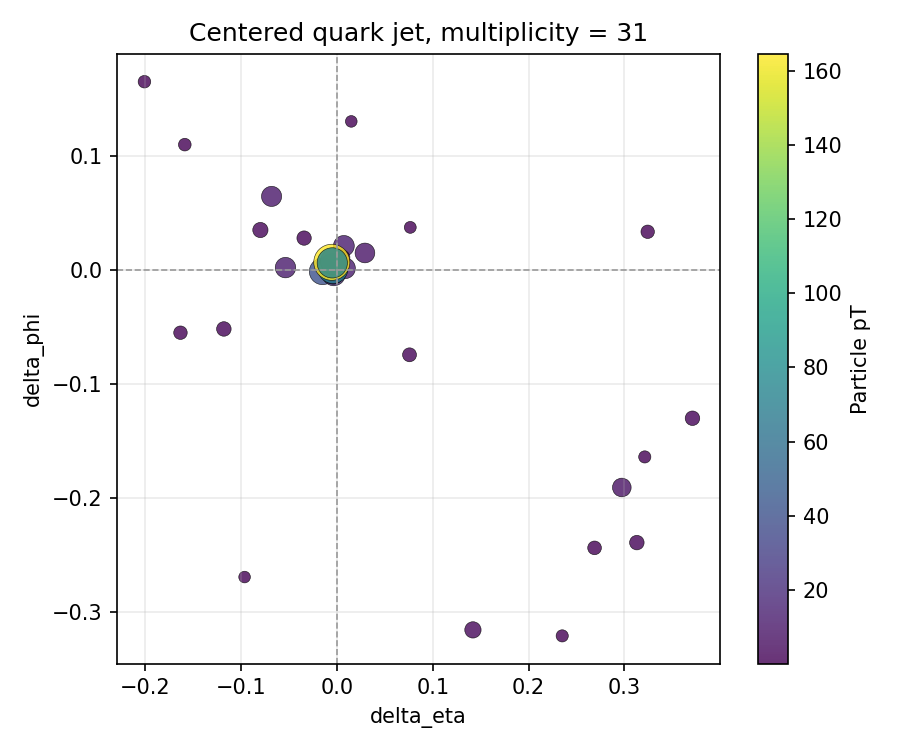
\includegraphics[width=0.46\textwidth]{../figures/jet_display_quark_centered.png}
  \hfill
  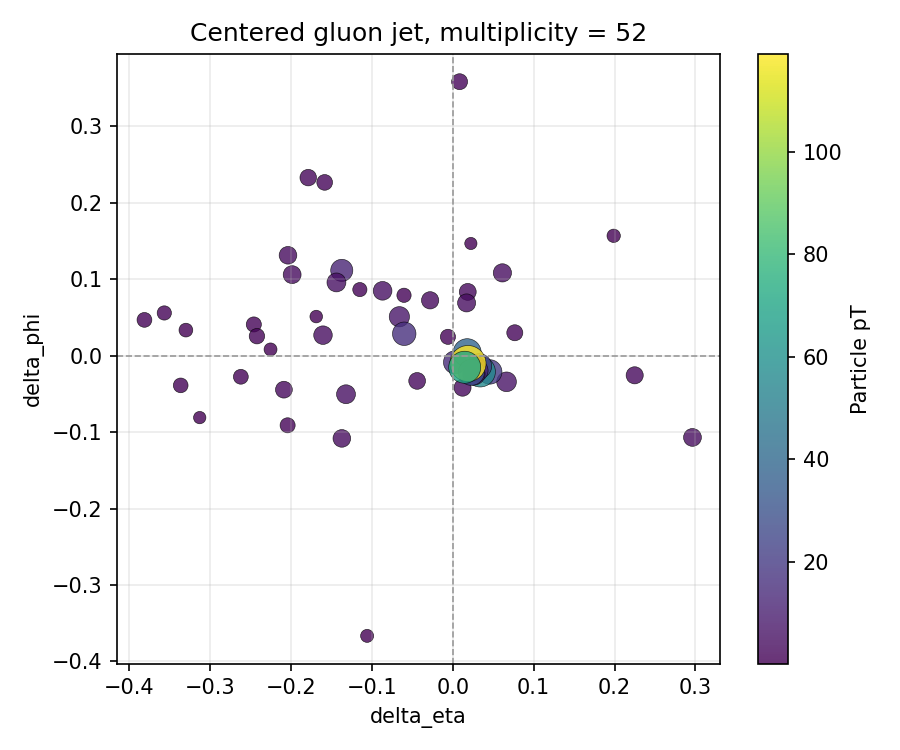
\includegraphics[width=0.46\textwidth]{../figures/jet_display_gluon_centered.png}
  \caption{Centered quark and gluon jet displays in
  $(\Delta\eta,\Delta\phi)$ coordinates. Marker size is proportional to particle
  transverse momentum.}
  \label{fig:jet-displays}
\end{figure}

\section{EdgeConv Architecture}

The first graph model is intentionally simple. It consists of two EdgeConv
layers with ReLU activations, followed by global mean pooling and a small MLP
classifier. The model is trained with cross-entropy loss for binary
classification. This minimal architecture is sufficient for controlled
experiments on feature representation and graph connectivity.

\section{Results}

\subsection{Baseline Comparison}

The observable-only baselines are already highly competitive, as shown in
Table~\ref{tab:baseline}. Gradient boosting reaches ROC AUC 0.8616.

\begin{table}[htbp]
  \centering
  \caption{Performance of physics-observable baseline classifiers.}
  \label{tab:baseline}
  \begin{tabular}{lc}
    \toprule
    Model & ROC AUC \\
    \midrule
    Logistic regression & 0.8579 \\
    Random forest & 0.8451 \\
    Gradient boosting & 0.8616 \\
    \bottomrule
  \end{tabular}
\end{table}

\begin{figure}[htbp]
  \centering
  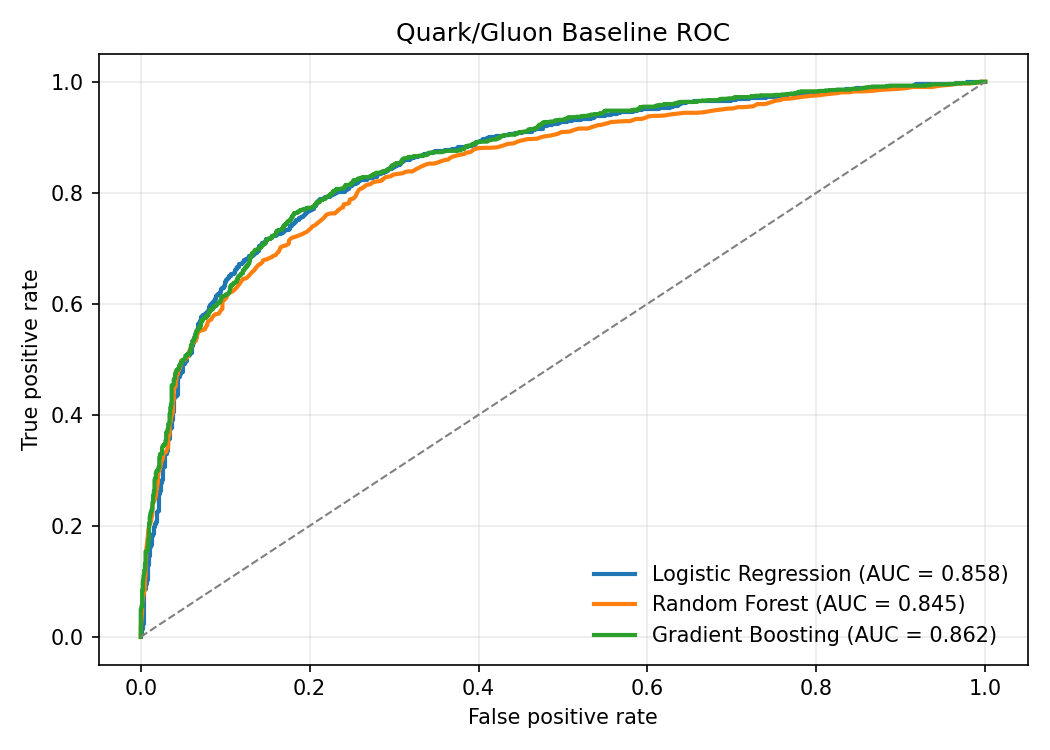
\includegraphics[width=0.74\textwidth]{../figures/baseline_roc.png}
  \caption{ROC curves for the physics-inspired baseline classifiers.}
  \label{fig:baseline-roc}
\end{figure}

\subsection{Feature Ablation}

The EdgeConv model is sensitive to node-feature representation. Raw features
already work well, physics-only relative features underperform, and hybrid
features recover the best performance.

\begin{table}[htbp]
  \centering
  \caption{EdgeConv node-feature ablation.}
  \label{tab:feature-ablation}
  \begin{tabular}{lc}
    \toprule
    Feature mode & ROC AUC \\
    \midrule
    Raw & 0.8580 \\
    Physics & 0.8102 \\
    Hybrid & 0.8617 \\
    \bottomrule
  \end{tabular}
\end{table}

\begin{figure}[htbp]
  \centering
  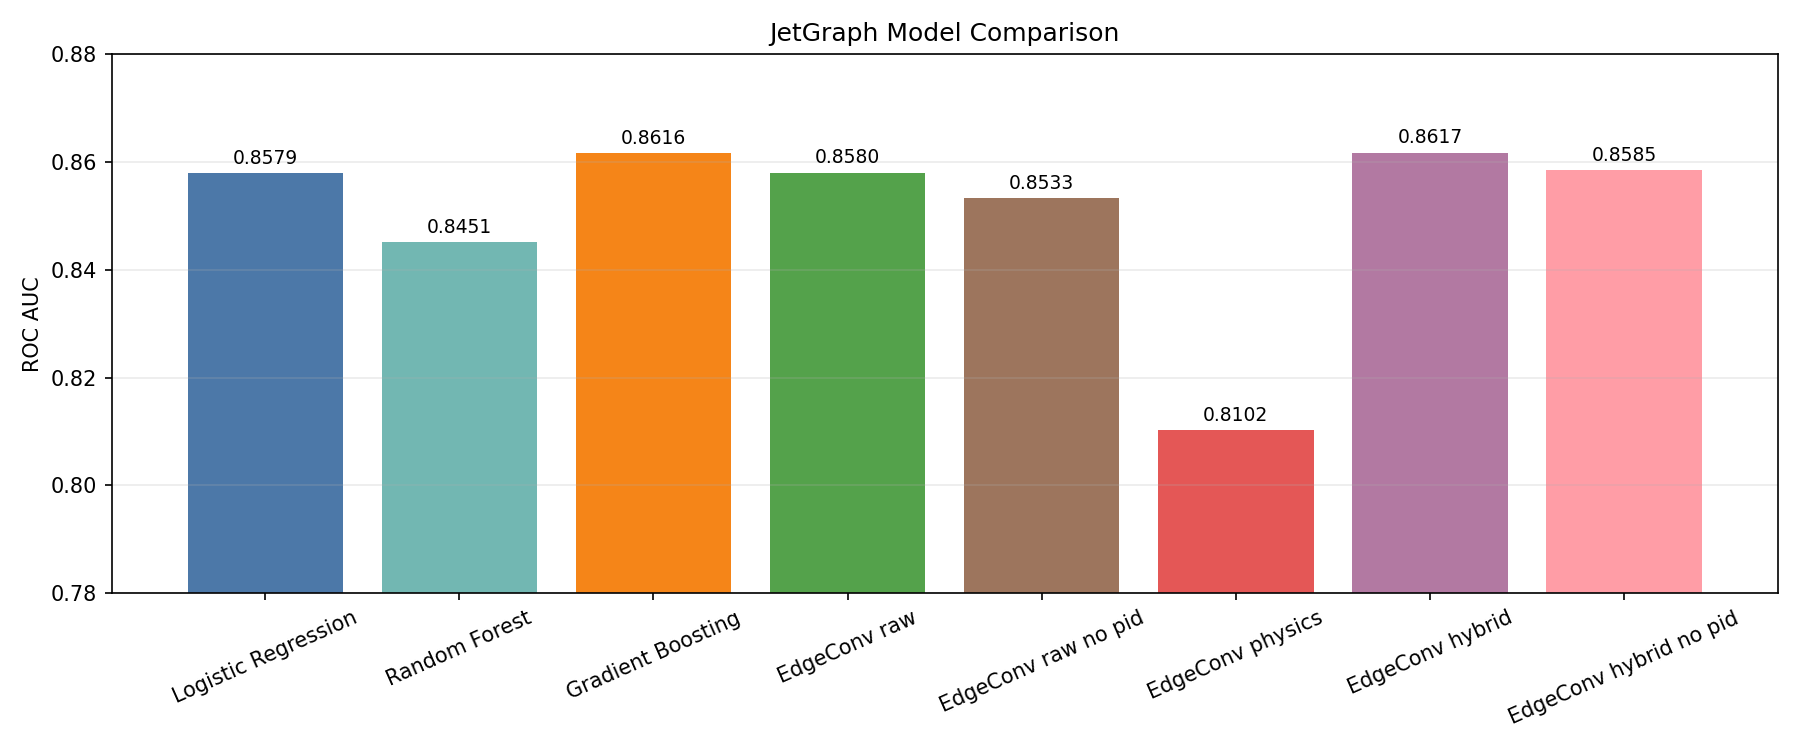
\includegraphics[width=0.88\textwidth]{../figures/model_comparison.png}
  \caption{Summary of baseline and EdgeConv model comparisons.}
  \label{fig:model-comparison}
\end{figure}

\subsection{k-Connectivity Study}

Using hybrid node features, the graph connectivity parameter is scanned over
$k=4,8,12,16$. The best AUC in this sweep is obtained at $k=8$.

\begin{table}[htbp]
  \centering
  \caption{Impact of the k-nearest-neighbour connectivity parameter.}
  \label{tab:k-study}
  \begin{tabular}{ccc}
    \toprule
    $k$ & Test accuracy & Test ROC AUC \\
    \midrule
    4 & 0.7653 & 0.8525 \\
    8 & 0.7707 & 0.8579 \\
    12 & 0.7720 & 0.8511 \\
    16 & 0.7640 & 0.8455 \\
    \bottomrule
  \end{tabular}
\end{table}

\begin{figure}[htbp]
  \centering
  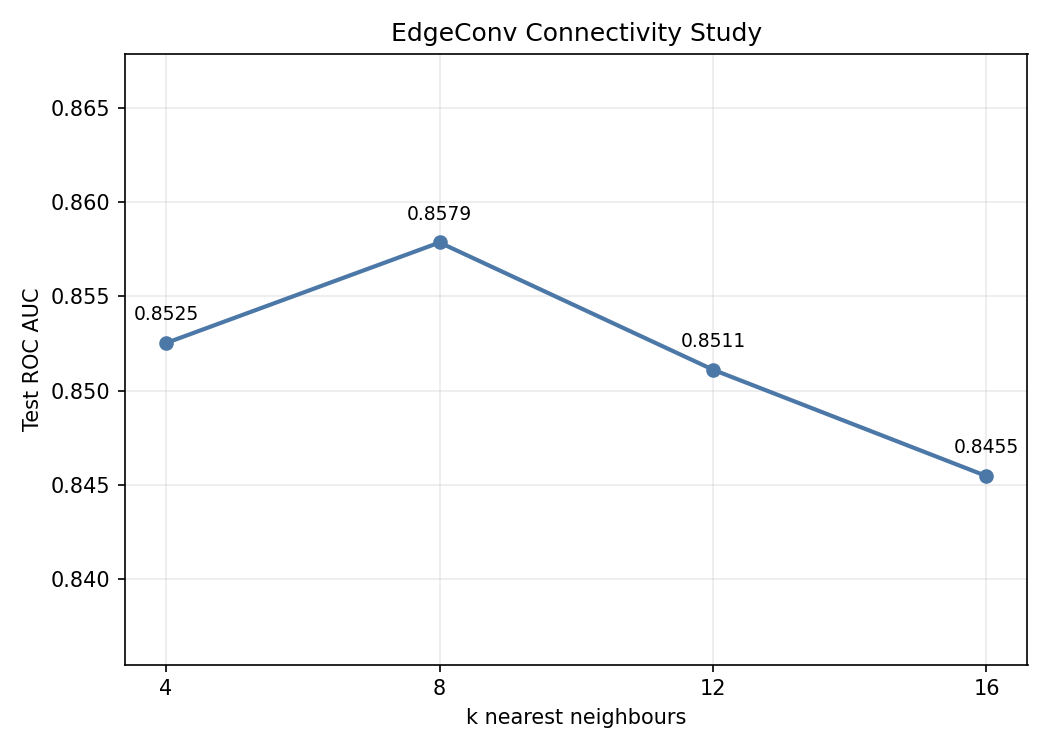
\includegraphics[width=0.72\textwidth]{../figures/k_study_auc.png}
  \caption{Test ROC AUC as a function of kNN graph connectivity.}
  \label{fig:k-study}
\end{figure}

\subsection{pid/no-pid Study}

Particle identity information provides a small but visible gain. Removing
\texttt{pid} lowers the raw-feature AUC from 0.8580 to 0.8533 and the
hybrid-feature AUC from 0.8617 to 0.8585.

\begin{table}[htbp]
  \centering
  \caption{Effect of removing particle identity from node features.}
  \label{tab:pid-study}
  \begin{tabular}{lcc}
    \toprule
    Feature family & With pid & Without pid \\
    \midrule
    Raw & 0.8580 & 0.8533 \\
    Hybrid & 0.8617 & 0.8585 \\
    \bottomrule
  \end{tabular}
\end{table}

\subsection{Generator Robustness}

The generator-robustness study trains on one generator and tests on both Pythia
and Herwig~\cite{sjostrand2015pythia,bellm2016herwig}. The results in
Table~\ref{tab:generator} show a significant drop when a Pythia-trained model is
evaluated on Herwig.

\begin{table}[htbp]
  \centering
  \caption{Pythia-vs-Herwig generator robustness.}
  \label{tab:generator}
  \begin{tabular}{llcc}
    \toprule
    Train generator & Test generator & Accuracy & ROC AUC \\
    \midrule
    Pythia & Pythia & 0.7707 & 0.8579 \\
    Pythia & Herwig & 0.7147 & 0.7835 \\
    Herwig & Pythia & 0.7693 & 0.8464 \\
    Herwig & Herwig & 0.7053 & 0.7955 \\
    \bottomrule
  \end{tabular}
\end{table}

\begin{figure}[htbp]
  \centering
  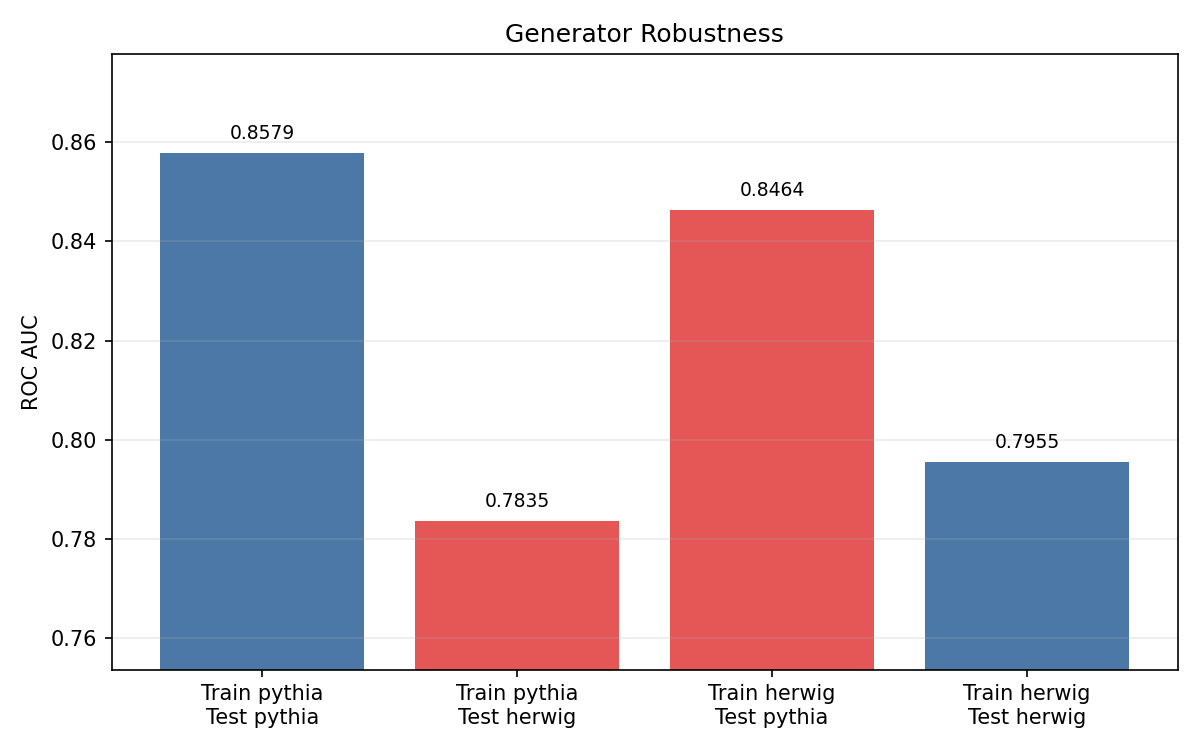
\includegraphics[width=0.74\textwidth]{../figures/generator_robustness.png}
  \caption{Cross-generator ROC AUC comparison for EdgeConv models trained on
  Pythia or Herwig.}
  \label{fig:generator}
\end{figure}

\section{Discussion}

The study demonstrates that simple physically motivated observables remain a
strong baseline for quark/gluon tagging. The EdgeConv graph model reaches
similar performance only after careful feature design. In particular, removing
absolute kinematic information in the physics-only representation degrades the
result, while hybrid features combining absolute and relative coordinates
perform best.

The graph-connectivity scan suggests that moderately local neighbourhoods are
useful, but denser graphs do not automatically improve performance. The
generator study is the main cautionary result: strong in-domain performance does
not imply robust physics learning across different Monte Carlo generators.

\section{Conclusion and Future Work}

JetGraph provides a concise, reproducible mini-study of graph learning for
quark--gluon tagging. The best current EdgeConv result, ROC AUC 0.8617 with
hybrid node features, is comparable to the best gradient-boosted observable
baseline. This confirms both the strength of traditional physics-inspired
variables and the potential of graph-based representations.

Future work should study larger samples, repeated random seeds, train-set-only
feature normalization, dynamic graph recomputation, and ParticleNet-like
architectures. The most important next step is to improve Pythia-vs-Herwig
robustness, for example with mixed-generator training or domain-adversarial
objectives.

\bibliographystyle{unsrt}
\bibliography{references}

\end{document}
